
\section{On blockchain voting}
Will blockchain create the base technology for democratic applications? The answer is still outstanding. A lot of questions arise regarding both the voting process and the underlying technology. A lot of them remain unanswered. This paper tries to ask all questions and -- where possible -- gather and evaluate potential approaches to solve them.

\subsection{Why blockchain matters}
After Satoshi Nakamoto presented the first concept of a fully decentralized and trustless currency \textsc{Bitcoin (BTC)} in 2008 [NAKAMOTO~2008] and published the first blockchain protocol reference implementation in 2009, many years have passed until the underlying technology seriously got recognized as a game changer by the technology scene. Blockchain tools today are considered and valued with a high potential. The current emerge of blockchain related start-ups aswell as global operating coorperations entering the market is often compared to the beginning of the internet [ÉPIÉ~et~al.~2015].\par
The impact on society, industry and governance hardly can be estimated. Suddenly, transactions can share information without any middle man. The blockchain is owned, run  and monitored by everyone, but controlled by anyone [ÉPIÉ~et~al.~2015].\par
The non-hierarchical, self-organizing, peer-to-peer collaboration nature of blockchain ecosystems within communitarian network structures is the foundation for both censorship resistance and full transparency, which leaves no room for any tampering. This is a big feature that nothing but blockchains can provide [SCOTT~2016] [KAYE~2016].

\subsection{Blockchain 2.0 technology}
In 2013 so called \textit{Bitcoin 2.0} projects or \textit{blockchain 2.0} technologies emerged. They aim is to provide collectively maintained decentralized ledgers that record things other than currency transactions and store all manner of diverse data, including voting decisions [SCOTT~2016].\par
At the cutting edge of the scene are smart contracts, small scripts on the blockchain, which participants can interact with. The new contract-orientated development paradigm allows for a switch in terminology: the \textit{trustless} nature of transactions on the blockchain moves aside for \textit{trust-enabling} transparent scripts doing exactly as programmed [SCOTT~2016].\par
% smart contracts: automatically execute the conditions and terms [ÉPIÉ~et~al.~2015]
% virtual, autonomous, without central control, trustable [ÉPIÉ~et~al.~2015]
Among the most innovative blockchain 2.0 technologies of the recent years are \textsc{Bitshares (BTS)}, \textsc{Ripple (XRP)}, \textsc{Nxt (NXT)} and \textsc{Ethereum (ETH)}.\par % @TODO Stellar, Tendermint, Hyperledger
Bitshares offers a stack of financial services including exchange and banking on a blockchain. It is mainly trageted at next-level financial applications and developed the concept of decentralized autonomous coorperations (\textsc{DAC}) which operate autonomous on the blockchain, issue tokes and payout shareholders as programmed.\par
Ripple is a commercial solution for the financial technology sector. Its distributed financial technology allows for banks to directly transact with each other without the need for a central counterparty or correspondent.\par
% @TODO check for relevance Stellar, Tendermint, Hyperledger
Nxt improves the financial technology, crowdfunding and governance industries by providing powerful, modular toolsets to build any application on top of the blockchain.\par
Blockchain 2.0 projects are often considered to pave the way for the \textit{Web 3.0} which will be decentralized. Ethereum claims to be \enquote{the way the internet was supposed to work}. \enquote{What Bitcoin does for payments, Ethereum does for anything that can be programmed.}, states Grace Caffyn from Coindesk referring to the underlying technology.\par
%\begin{figure}[H]
%\centering
%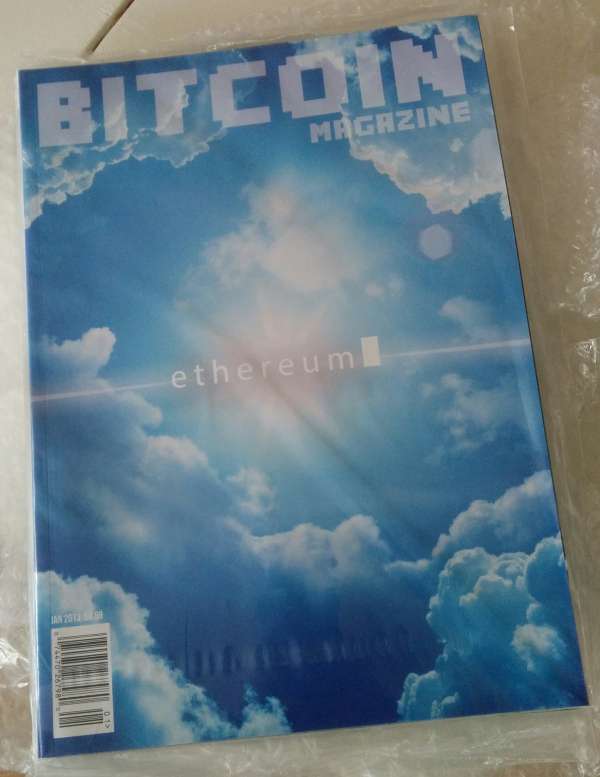
\includegraphics[draft,width=0.3\textwidth]{img/bitmag.png}
%\caption{The Bitcoin Magazine January 2014 Issue: On Ethereum.}
%\label{fig:mag}
%\end{figure}
The Ethereum blockchain contains a distributed virtual machine (\textsc{EVM}) which enables code on the blockchain to be executed. Whereas every blockchain technology offers it's own, often limited scripting languages, the revolutionary concept behind the EVM is the lifting of all limits by implementing a \textit{turing-complete} programming language. This allows -- in theory -- to build everything on top of the Ethereum blockchain technology: Smart contracts implement the logic, the blockchain manages the decentralized consensus and users can interact with trustable decentralized applications (\textsc{DApps}) [ÉPIÉ~et~al.~2015].

\subsection{Blockchain voting versus \enquote*{votechains}}
Voting is a key functionality of blockchain technology. The underlying consensus protocols on most distritubted peer-to-peer solutions always have to include ways to update protocols and restore consensus upon disputes. A prominent example is the Bitcoin Improvement Proposal \#BIP34, of the crypto-currency \textsc{Bitcoin} [NAKAMOTO~2008], proposing miner behaviour on softforking mechanics. This is voting on a very technical level and not considered part of this paper.\par
The following projects and voting references rather focus on applications or services \textit{on top of} blockchains, enabling democratic participation in any kind of groups, communities or societies.

\subsection{Requirements for voting applications}
\label{sec:req}
Electronic or online voting has to follow the same high standards as traditional paper or offline voting processes do. Necessary key feauteres and requirements will be gathered below. Existing approaches to blockchain based voting applications will be checked against these criteria.\par
How can elections be auditable and anonymous? How can a voter's identity be private but verifiable? [VARSHNEYA~et~al.~2015] aswell as [ERNEST~2016] and [BORGSTRUP~2014] define following key features for blockchain voting.
\begin{itemize}
\item \textbf{Fair}. Participants can vote for anyone they like, not only the candidate they prefer most.
\item \textbf{Accessible}. Everyone should be able to use it without the introduction of any entry barriers.
\item \textbf{Anonymous}. Privacy of voters has to be protected and it should be infeasable to determine identity behind a vote. % @TODO sybil
\item \textbf{Authenticated}. The identity on the blockchain must be unique, and provable certified to vote to ensure only registered voters can take part in elections.
\item \textbf{Secure}. It also has to be impossible to decrypt voter's identities or to link voter's to voting behaviour. All communications should be encrypted.
\item \textbf{Integer}. It should not be possible to tamper with votes.
\item \textbf{Coercion-resistant}. The system should be able to prevent coercion of voters to vote in a certain way.
\item \textbf{Verifiable}. Individuals must be able to verify their votes are included in the final tally. Also, anyone must be able to check the election results were computed correctly.
\item \textbf{Auditable}. The whole process must enable a complete audit trail from the first user authentication through the final election.
\item \textbf{Decentralized}. A trust-enabling and tamper-resistant blockchain voting system has to be decentralized by design.
\item \textbf{Open source}. It has to be possible to examine code and to verify everything works as proposed.
\end{itemize}
Only applications fullfilling all points above should be considered for official electronic voting processes. % TODO OPEN SOURCE: Proposed solutions which fail to deliver open source products will be automatically applied a zero score as they are impossible to peer review.
